\subsection{M.PC.9 - Frequenza di merge delle pull request}
\begin{figure}[H]
    \centering
    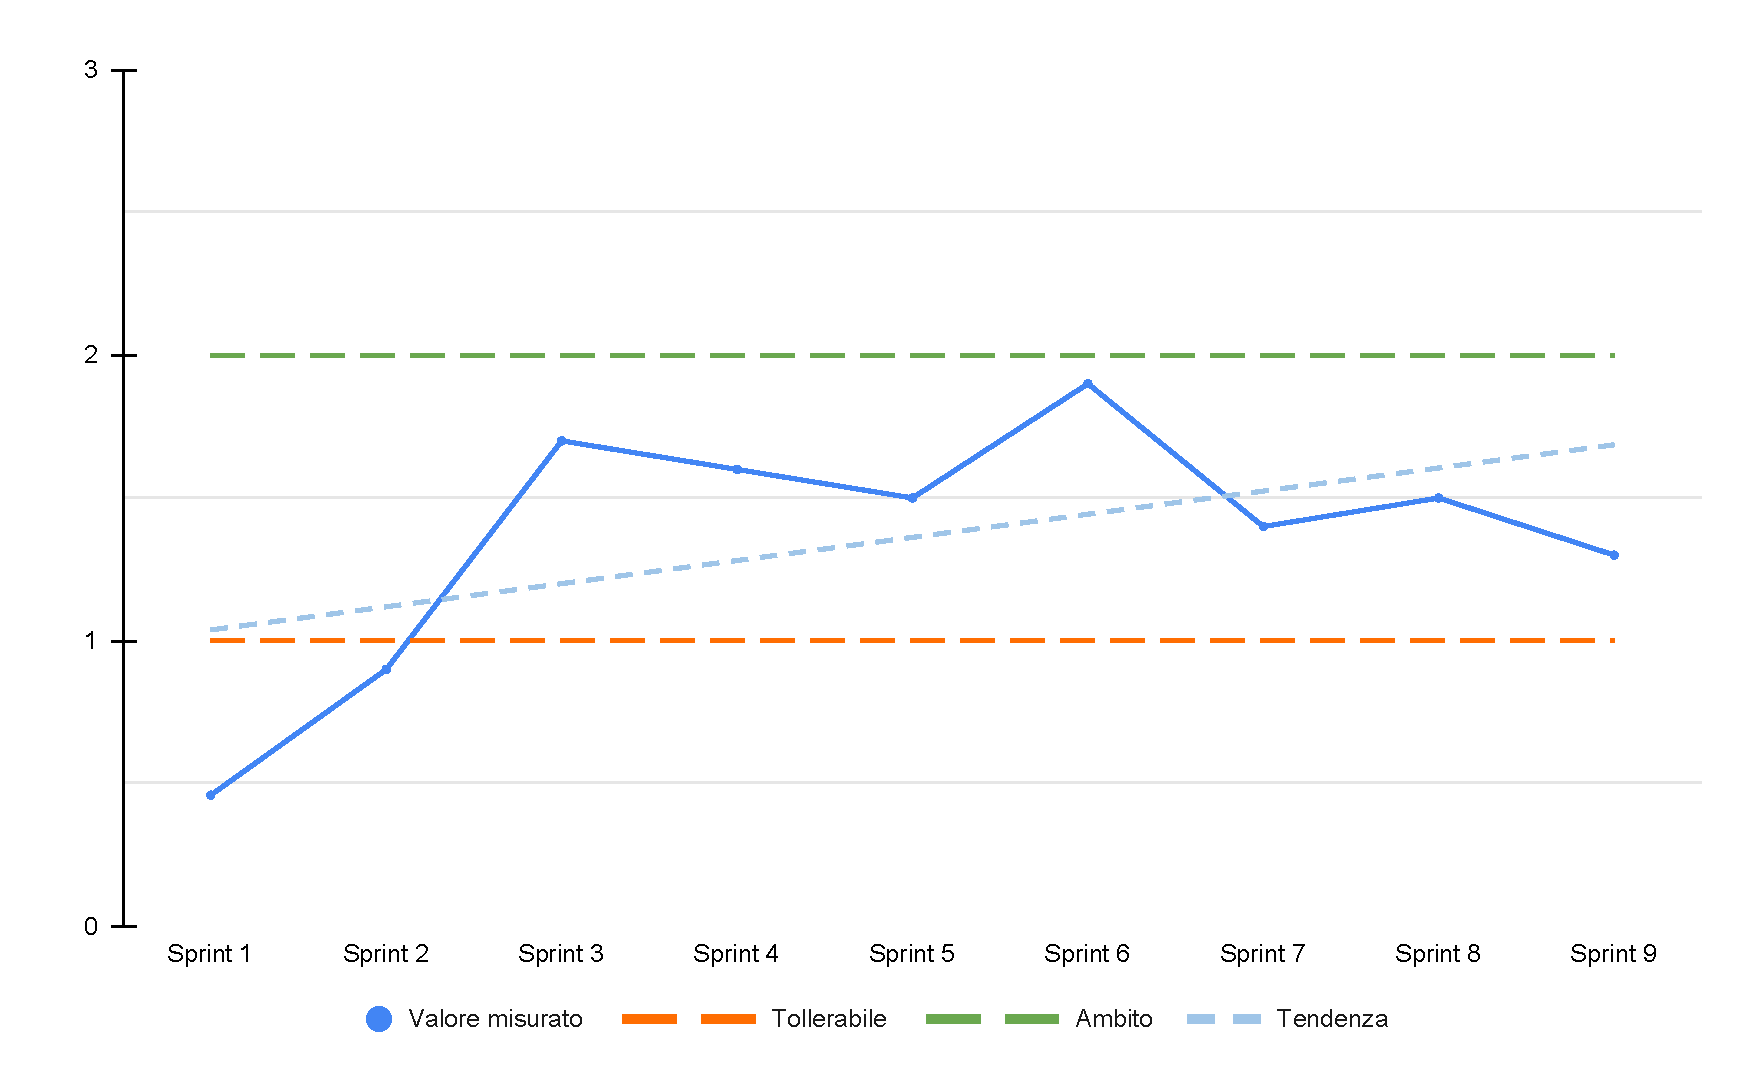
\includegraphics[width=\textwidth]{assets/frequenza_pull_request.pdf}
    \caption{M.PC.9 - Frequenza di merge delle pull request}
\end{figure}

\par Nei primi due \glossario{sprint}, la frequenza di merge delle pull request è stata inferiore alle aspettative; questo è dovuto al fatto che, nelle fasi iniziali del progetto, gli sforzi del gruppo si sono concentrati sulla produzione di documenti. Data l’inesperienza del team nella stesura della documentazione, le pull request sono state aperte con discontinuità. Inoltre, la portata delle modifiche ha rallentato il processo di verifica e approvazione. Pertanto, la frequenza di merge non ha raggiunto il valore tollerabile (1 volta al giorno). Il team ha quindi deciso di ridurre il valore ambito, da 3 volte al giorno a 2. Dal terzo sprint, vista la necessità di aggiornare specifiche sezioni dei documenti, il gruppo ha ritenuto opportuno integrare le modifiche con maggior frequenza. È stata introdotta la pratica di \glossario{continuous integration}, migliorando il processo di allineamento delle modifiche e consentendo verifiche rapide e frequenti. Un fattore che ha contribuito a incrementare la frequenza di merge è stato lo sviluppo del \glossario{PoC}, le cui funzionalità sono state suddivise in task di dimensioni ridotte, al fine di promuovere l'integrazione continua. Grazie all’applicazione di questa contromisura, il team ha mantenuto un flusso di lavoro regolare. Come testimonia il grafico, i valori misurati a partire dal terzo sprint rientrano nel range di tollerabilità stabilito. In concomitanza del sesto sprint, la frequenza di merge delle pull request si è avvicinata al valore ambito; considerando il cambio di tecnologie avvenuto nell’iterazione precedente, questo risultato dimostra l’efficacia delle strategie adottate dal gruppo.
